\documentclass[compress,mathserif]{beamer}
\usetheme{sthlm}

%-=-=-=-=-=-=-=-=-=-=-=-=-=-=-=-=-=-=-=-=-=-=-=-=
%        LOADING BEAMER PACKAGES
%-=-=-=-=-=-=-=-=-=-=-=-=-=-=-=-=-=-=-=-=-=-=-=-=

\usepackage{
booktabs,
datetime,
dtk-logos,
graphicx,
multicol,
pgfplots,
ragged2e,
tabularx,
tikz,
wasysym,
multirow,
float,
caption,
subcaption,
amsmath,
mathptmx,
animate
}

\usepackage[scaled=0.9]{helvet}
\usepackage{courier}

\usefonttheme[onlymath]{serif}

\definecolor{mygreen}{RGB}{113, 166, 70}
\definecolor{myblue}{RGB}{68, 140, 185}
\definecolor{myred}{RGB}{217, 98, 55}
\definecolor{mypurple}{RGB}{83, 65, 126}
\definecolor{solviaveis}{RGB}{188, 207, 241}

\pgfplotsset{compat=1.8}

\usepackage[utf8]{inputenc}
\usepackage[portuguese]{babel}
\usepackage[T1]{fontenc}
\usepackage{newpxtext,newpxmath}
\usepackage{listings}

\lstset{ %
language=[LaTeX]TeX,
basicstyle=\normalsize\ttfamily,
keywordstyle=,
numbers=left,
numberstyle=\tiny\ttfamily,
stepnumber=1,
showspaces=false,
showstringspaces=false,
showtabs=false,
breaklines=true,
frame=tb,
framerule=0.5pt,
tabsize=4,
framexleftmargin=0.5em,
framexrightmargin=0.5em,
xleftmargin=0.5em,
xrightmargin=0.5em
}



%-=-=-=-=-=-=-=-=-=-=-=-=-=-=-=-=-=-=-=-=-=-=-=-=
%        LOADING TIKZ LIBRARIES
%-=-=-=-=-=-=-=-=-=-=-=-=-=-=-=-=-=-=-=-=-=-=-=-=

\usetikzlibrary{
backgrounds,
mindmap
}

%-=-=-=-=-=-=-=-=-=-=-=-=-=-=-=-=-=-=-=-=-=-=-=-=
%        BEAMER OPTIONS
%-=-=-=-=-=-=-=-=-=-=-=-=-=-=-=-=-=-=-=-=-=-=-=-=

\setbeameroption{show notes}

%-=-=-=-=-=-=-=-=-=-=-=-=-=-=-=-=-=-=-=-=-=-=-=-=
%        BEAMER COMMANDS
%-=-=-=-=-=-=-=-=-=-=-=-=-=-=-=-=-=-=-=-=-=-=-=-=


%-=-=-=-=-=-=-=-=-=-=-=-=-=-=-=-=-=-=-=-=-=-=-=-=
%
%	PRESENTATION INFORMATION
%
%-=-=-=-=-=-=-=-=-=-=-=-=-=-=-=-=-=-=-=-=-=-=-=-=

\title{Representação algébrica de problemas de Programação Linear}
\subtitle{DCE692 - Pesquisa Operacional}
%\date{\small{\jobname}}
\author{\texttt{Iago Carvalho}}
\institute{\texttt{Departamento de Ciência da Computação}}

\hypersetup{
pdfauthor = {Iago A. Carvalho},      
pdfsubject = {Pesquisa Operacional},
pdfkeywords = {},  
pdfmoddate= {D:\pdfdate},          
pdfcreator = {WriteLaTeX}
}

\begin{document}

\begin{frame}
\titlepage

\end{frame}

%% --------------------------------------------------------

\begin{frame}{Programação Linear}

Problemas de programação linear são descritos utilizando um conjunto de equações lineares
\begin{itemize}
    \item Função objetivo
    \item Variáveis
    \item Restrições
\end{itemize}

\vspace{0.5cm}

É possível representar graficamente um problema de programação linear
\begin{itemize}
    \item 3 variáveis
    \item Poucas restrições
\end{itemize}

\vspace{0.5cm}

E problemas maiores?
\end{frame}

%% --------------------------------------------------------

\begin{frame}{Programação Linear - Representação matricial}

De forma geral, um problema de programação linear é representado como

  $$\begin{matrix}
        \min & c^Tx \\ 
             & Ax & \leqslant b \\
             & x & \geqslant 0 
        \end{matrix}    
$$

onde 
\begin{columns}[T]
    \begin{column}{.49\textwidth}
    $$A = \begin{bmatrix}
a_{11} & a_{12} & \dots & a_{1n}\\ 
a_{21} & a_{22} & \dots & a_{2n}\\ 
\vdots & \vdots & \ddots & \vdots \\ 
a_{m1} & a_{m2} & \dots & a_{mn}
\end{bmatrix}$$
\end{column}
    \begin{column}{.49\textwidth}
    \vspace{0.55cm}
    $c = \{c_1, c_2, \ldots, c_n\}$ \\
    \vspace{0.25cm}
    $x^T = \{x_1, x_2, \ldots, x_n\}$ \\
    \vspace{0.25cm}
    $b^T = \{b_1, b_2, \ldots, b_m\}$
    \end{column}
\end{columns}
\end{frame}

%% --------------------------------------------------------

\begin{frame}{Representação como somatórios}


Representação matricial
    $$\begin{matrix}
        \min & c^Tx \\ 
             & Ax & \leqslant b \\
             & x & \geqslant 0 
        \end{matrix}    
$$
Representação com somatórios
    $$\begin{matrix}
        \min & \sum_{i = 1}^n c_i~x_i \\      & \sum_{i = 1}^n a_{ji}~x_i & \leqslant b_j, & \forall j \in \{1, 2, \ldots, m\}  \\
             & x_i & \geqslant 0 & \forall i \in \{1, 2, \ldots, n \}
        \end{matrix}    
$$
\end{frame}

%% --------------------------------------------------------

\begin{frame}{Representação matricial extendida}

Representação matricial
    $$\begin{matrix}
        \min & c^Tx \\ 
             & Ax & \leqslant b \\
             & x & \geqslant 0 
        \end{matrix}    
$$
Representação extendida

$$
\begin{matrix} 
\min & c_1 x_1 & + & c_2 x_2 & + & \dots & + & c_n x_n & \\
     & a_{11} x_1 & + & a_{12} x_2 & + & \dots  & + & a_{1n} x_n & \leqslant & b_1 \\
     & a_{21} x_1 & + & a_{22} x_2 & + & \dots  & + & a_{2n} x_n & \leqslant & b_2 \\
     & \vdots     &   & \vdots     &   & \ddots &   & \vdots     &           & \vdots \\
     & a_{m1} x_1 & + & a_{m2} x_2 & + & \dots  & + & a_{mn} x_n & \leqslant & b_m \\
     & x_1,       &   & x_2,       &   & \dots  &   &        x_n & \geqslant & 0 \\
\end{matrix}
$$
\end{frame}

%% --------------------------------------------------------

\begin{frame}{Variáveis de folga}

Representação matricial
    $$\begin{matrix}
        \min & c^Tx \\ 
             & Ax + y & = b \\
             & x & \geqslant 0 \\
             & y & \geqslant 0
        \end{matrix}    
$$
Representação extendida

\centering 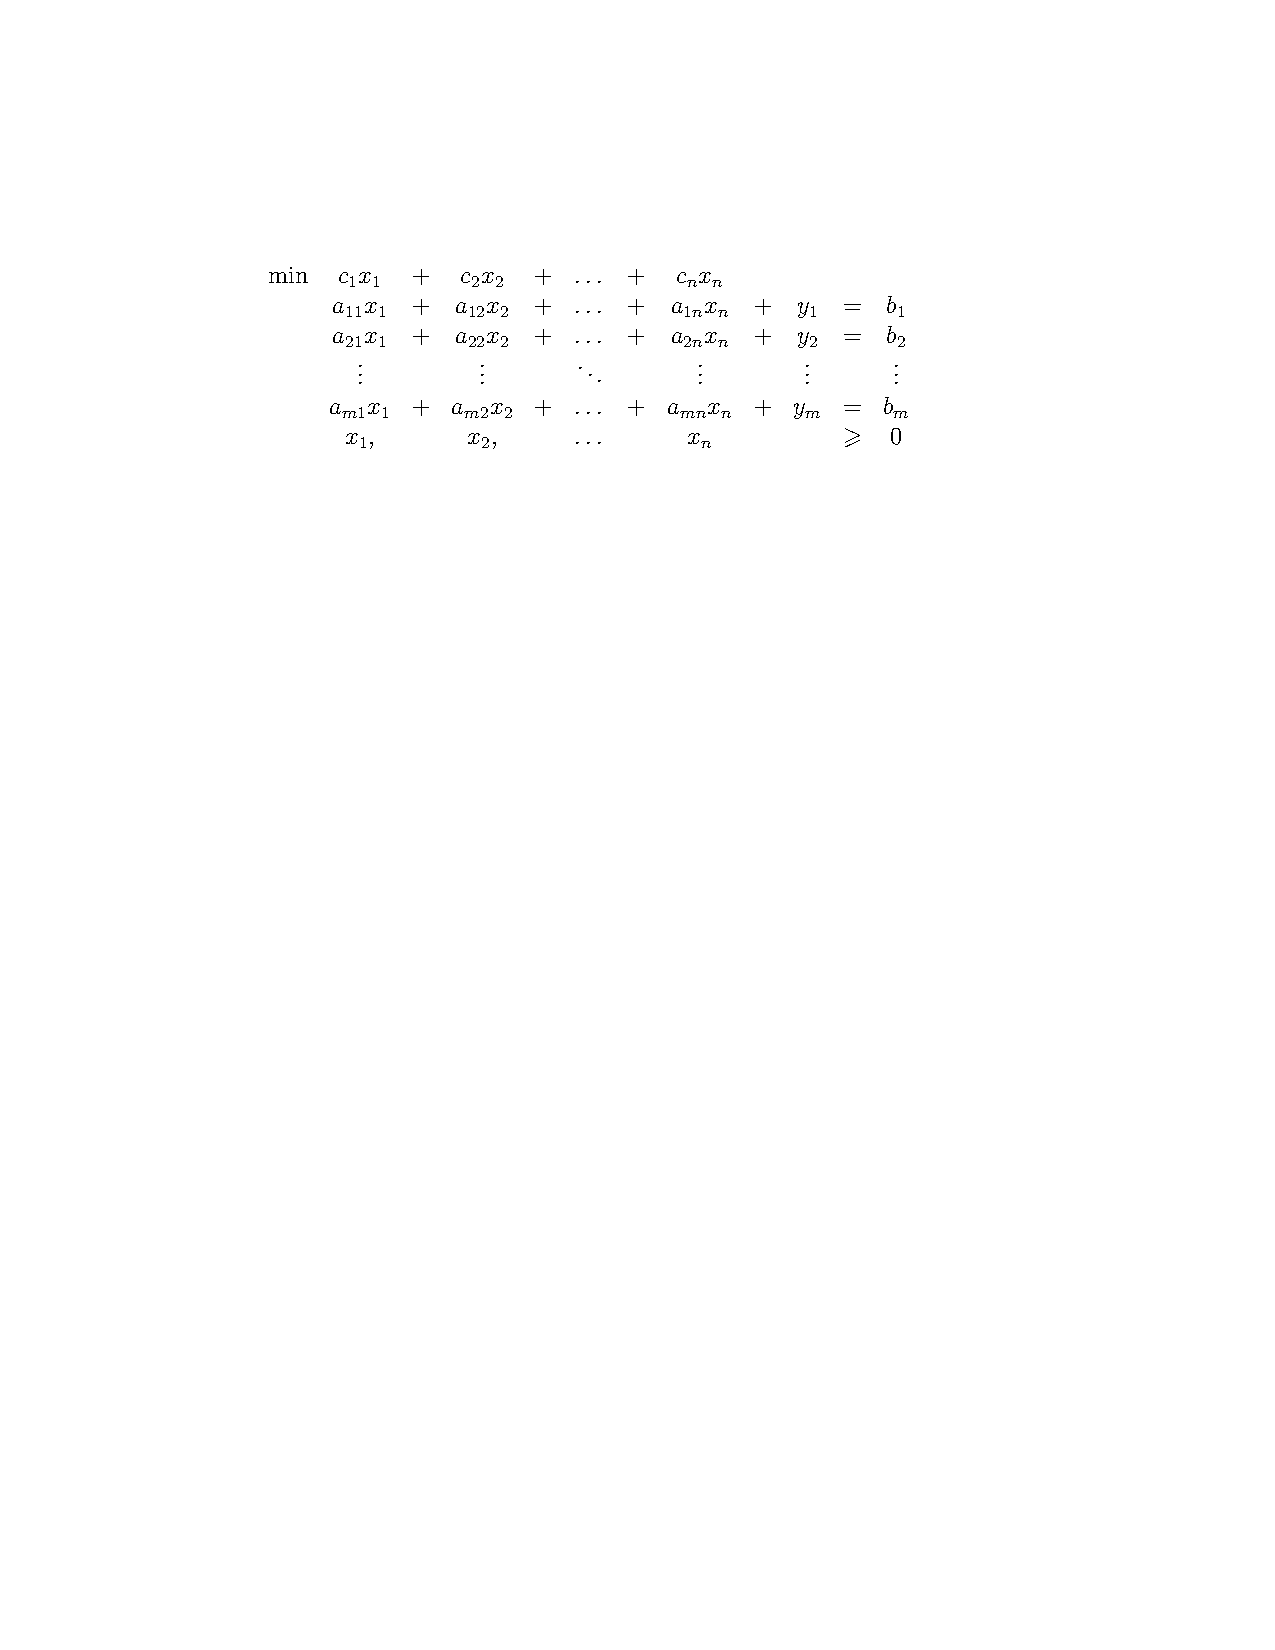
\includegraphics[width=\textwidth]{images/equation.pdf}
\end{frame}

% A formula¸c˜ao de um modelo geral de programa¸c˜ao linear pode ser
% representada matematicamente como:
% max ou mim z = f (x1, x2, . . . xn) = c1x1 + c2x2 + · · · + cnxn
% sujeito a: a11x1 + a12x2 + · · · + a1nxn{ ≤=≥ }b1
% : : :
% am1x1 + am2x2 + · · · + amnxn{ ≤=≥ }bm
% x1, x2, . . . , xn ≥ 0
% em que z ´e a fun¸c˜ao objetivo; xj
% , j = 1, 2, . . . , n s˜ao as vari´aveis de
% decis˜ao; ai
% j, i = 1, 2, . . . , m ´e a constante da i-´esima restri¸c˜ao da j-´esima
% restri¸c˜ao; bi ´e o termo independente ou quantidade de recursos dispon´ıveis
% da i-´esima restri¸c˜ao; e cj ´e a constante ou coeficiente da j-´esima vari´avel
% da fun¸c˜ao objetivo.


\end{document}